\documentclass[12pt]{article}
%\usepackage[english]{babel}
\RequirePackage[spanish]{babel}
\usepackage[spanish]{babel}
\usepackage{graphicx}
\usepackage[pdftex,bookmarks,colorlinks,breaklinks]{hyperref}  % PDF hyperlinks, with coloured links
%\usepackage[spanish]{babel}
\usepackage[utf8]{inputenc}
\usepackage{courier}
\usepackage{epstopdf}
\usepackage{fullpage}
\usepackage{url}
\usepackage{colortbl}
\usepackage{lscape}
\usepackage{xcolor}
\usepackage[skins,listings,breakable]{tcolorbox}
%\usepackage{listings}
\lstset{
  literate = {-}{-}1,
  basicstyle=\ttfamily\footnotesize,
  breaklines=true
}

\parskip 3ex % espacio entre parrafos.


\begin{document}
%%%%%%%%%%%%%%% PORTADA %%%%%%%%%%%%%%%%%%
\pagestyle{empty}
\begin{figure}
   \centering
   
\includegraphics[scale=.5]{imgs/logo.png}
\end{figure}

\begin{center}
Facultad de Ingeniería

Escuela de Ingeniería en Bioinformática

\bigskip\bigskip\bigskip\bigskip

\rule{14cm}{0.5mm}

\begin{Huge}\textbf{Informe Proyecto}\end{Huge}

\begin{Huge}\textbf{Administración de Sistemas}\end{Huge}

\rule{14cm}{0.5mm}

\bigskip\bigskip\bigskip\bigskip
\bigskip\bigskip\bigskip\bigskip
\bigskip\bigskip\bigskip\bigskip
\bigskip\bigskip\bigskip\bigskip


\begin{tabular*}{14cm}{l@{\extracolsep{\fill}}r}
\emph{Alumno:} & \emph{Profesor:}\\
Nicolás Rojas Poblete & Alejandro Valdés\\
\emph{Matrícula:} & \emph{Módulo:}\\
2016430002 & Administración de Sistemas\\
\emph{E-mail:} & \emph{Minor:}\\
nicrojas16@alumnos.utalca.cl & Desarrollo de Software y\\
& Administración de Sistemas\\
\end{tabular*}
\end{center}

%%%%%%%%%%%%%%%%%%%%%%%%%%%%%%%%%%%%%%%
\newpage
\pagestyle{plain}
\tableofcontents

%%%%%%%%%%%%%%%%%%%%%%%%%%%%%%%%%%%%%%%
\newpage
\listoffigures 

%%%%%%%%%%%%%%%%%%%%%%%%%%%%%%%%%%%%%%%
%\newpage%
%\listoftables%

%%%%%%%%%%%%%%%%%%%%%%%%%%%%%%%%%%%%%%%
\newpage
\section{Introducción}


\newpage
\section{Compilando programas, librerías, kernel}

\subsection{Compilando el compilador GCC}

El compilador es muy importante dentro de los sistemas informáticos, se encargan de traducir el código fuente de los programas a un lenguaje que pueda ejecutar la máquina. En sistemas Linux por lo general viene incluído el compilador GCC en una versión defecto. Para ver la versión por defecto se puede ejecutar el siguiente comando.

\begin{lstlisting}[frame=single,framexrightmargin=15pt]
$ gcc --version
gcc (Debian 8.3.0-6) 8.3.0
Copyright (C) 2018 Free Software Foundation, Inc.
This is free software; see the source for copying conditions.  There is NO
warranty; not even for MERCHANTABILITY or FITNESS FOR A PARTICULAR PURPOSE.
\end{lstlisting}

En caso de que no se encuentre instalado, se puede instalar desde los repositorios de su distribución por apt u otro gestor de paquetes.

\begin{lstlisting}[frame=single,framexrightmargin=15pt]
$ sudo apt install gcc
\end{lstlisting}

\subsubsection{Prerequisitos GCC 9.3}

En este caso se procederá a instalar la versión 9.3 de GCC a partir de la versión 8.3 que viene en nuestro sistema instalada.

Según el sitio web de manualinux.eu\cite{mlinux} los requisitos para compilar gcc 9.3 son los siguientes:

\begin{lstlisting}[frame=single,framexrightmargin=15pt]
Gawk - (5.0.1)
M4 - (1.4.18)
Libtool - (2.4.6)
Make - (4.3)
Bison - (3.5.3)
Flex - (2.6.4)
Automake - (1.16.1)
Autoconf - (2.69)
Gettext - (0.20.1)
Gperf - (3.1)
Texinfo - (6.7)
\end{lstlisting}
\bigskip
\bigskip
\begin{lstlisting}[frame=single,framexrightmargin=15pt]
Librerias en Desarrollo

Gmp - (6.2.0)
Mpfr - (4.0.2)
Mpc - (1.1.0)
ISL - (0.18)
\end{lstlisting}

\subsubsection{Descarga y Configuración GCC 9.3}

Una vez revisadas las dependencias se procede a descargar el código fuente de GCC 9.3, esto en el ftp oficial.

\begin{lstlisting}[frame=single,framexrightmargin=15pt]
$ wget ftp://ftp.mirrorservice.org/sites/sourceware.org/pub/gcc/releases/gcc-9.3.0/gcc-9.3.0.tar.gz
\end{lstlisting}

Para descomprimir
\begin{lstlisting}[frame=single,framexrightmargin=15pt]
$ tar -xzvf gcc-9.3.0.tar.gz
\end{lstlisting}

Luego es necesario entrar en la carpeta y dentro de los archivos viene incluido un script que descarga las principales dependencias(Gmp,Mpfr,Mpc,ISL).

\begin{lstlisting}[frame=single]
$ cd gcc-9.3.0/
$ contrib/download_prerequisites
\end{lstlisting}

Luego se puede crear una carpeta aparte en dónde se configure y construya el nuevo compilador.

\begin{lstlisting}[frame=single]
$ cd ~
$ mkdir build-gcc9.3
$ cd build-gcc9.3/
\end{lstlisting}

Ahora se procede a ejecutar el ./configure con los siguiente parámetros.
\begin{lstlisting}[frame=single]
$ ../gcc-9.3.0/configure --build=x86_64-linux-gnu --host=x86_64-linux-gnu \
--target=x86_64-linux-gnu --enable-shared --enable-threads=posix \
--enable-__cxa_atexit --enable-clocale=gnu --enable-languages=c,c++,fortran \
--prefix=/usr/local/gcc-9.3 --disable-multilib --program-suffix=-9.3
\end{lstlisting}


\subsubsection{Instalación GCC 9.3}

Una vez terminada la configuración y creado el archivo make file se procede a compilar

\begin{lstlisting}[frame=single]
$ make -j 16
\end{lstlisting}
En este caso -j 16 indica la cantidad de CPUs disponibles en el sistema para la compilación. Dependiendo de la potencia puede tardar unos pocos minutos hasta un par de horas.

En este caso un CPU con 8 núcleos/16 hilos a 5.0 GHz la compilación solo tardó 15 minutos aproximadamente. 

\begin{lstlisting}[frame=single]
real    15m41.040s
user    140m26.060s
sys     3m52.618s
\end{lstlisting}

Luego como superusuario se copian los binarios al prefix indicado anteriormente en la configuración
\begin{lstlisting}[frame=single]
$ sudo make install-strip
\end{lstlisting}

Por último es necesario exportar el directorio a la variable de entorno PATH
\begin{lstlisting}[frame=single]
$ export PATH=$PATH:/usr/local/gcc-9.3/bin/
$ export export LD_LIBRARY_PATH=$LD_LIBRARY_PATH:/usr/local/gcc-9.3/lib64/
\end{lstlisting}

Ahora se puede comprobar la version instalada
\begin{lstlisting}[frame=single]
$ gcc-9.3 --version
gcc-9.3 (GCC) 9.3.0
Copyright (C) 2019 Free Software Foundation, Inc.
This is free software; see the source for copying conditions.  There is NO
warranty; not even for MERCHANTABILITY or FITNESS FOR A PARTICULAR PURPOSE.
\end{lstlisting}

\subsection{Compilando Librería KD-tree}

El primer paso es descargar el código fuente desde el repositorio oficial.
\begin{lstlisting}[frame=single]
$ wget http://nuclear.mutantstargoat.com/sw/kdtree/files/kdtree-0.5.7.tar.gz
$ tar -xzvf kdtree-0.5.7
$ cd kdtree-0.5.7/
\end{lstlisting}

Una vez listo se procede a configurar la librería y hacer la compilación.
\begin{lstlisting}[frame=single]
$ ./configure
$ make
\end{lstlisting}

\subsubsection{Creando Programa con la libraría KD-tree}

Se usa como base el ejemplo test2 incluido en el código fuente y se modifica para que solicite un punto inicial y el radio de búsqueda en el árbol. Quedando un programa como el siguiente.

\begin{tcblisting}{breakable,listing only,
  listing options={language=c,aboveskip=0pt,belowskip=0pt},
  size=fbox,boxrule=0pt,frame hidden,arc=0pt,colback=lightgray}
#include <assert.h>
#include <math.h>
#include <stdio.h>
#include <stdlib.h>
#include <ctype.h>
#include <time.h>
#include "kdtree.h"

#define DEF_NUM_PTS 10

/* entrega la distancia euclidiana entre 2 puntos */
static double dist_sq( double *a1, double *a2, int dims );

/* numero random entre -10 y 10 */
static double rd( void );

int main(int argc, char **argv) {
  printf("Kd-tree de 3 dimensiones\n");
  int i, num_pts = DEF_NUM_PTS;
  void *ptree;
  char *data, *pch;
  struct kdres *presults;
  double pos[3], dist;
  double pt[3];
  printf("Ingrese un numero de 3 dimensiones: (Separado por un espacio) ");
  scanf("%lf %lf %lf", &pt[0],&pt[1],&pt[2]);
  double radius;
  printf("Ingrese el radio de busqueda: ");
  scanf("%lf", &radius);
  if(argc > 1 && isdigit(argv[1][0])) {
    num_pts = atoi(argv[1]);
  }
  if(!(data = malloc(num_pts))) {
    perror("malloc failed");
    return 1;
  }
  srand( time(0) );
  /* Se crea el arbol kd-tree con 3 dimensiones */
  ptree = kd_create( 3 );
  /* Se agregan nodos con datos random al arbol */
  for( i=0; i<num_pts; i++ ) {
    data[i] = 'a' + i;
    assert( 0 == kd_insert3( ptree, rd(), rd(), rd(), &data[i] ) );
  }
  /* busca los nodos mas cercanos al punto entregado en el radio entregado por e                                                                                                                            l usuario */
  presults = kd_nearest_range( ptree, pt, radius );
  /* imprime los resultados */
  printf( "found %d results:\n", kd_res_size(presults) );

  while( !kd_res_end( presults ) ) {
    /* se obtiene las coordenadas de cada nodo con resultados */
    pch = (char*)kd_res_item( presults, pos );

    /* calcula la distancia euclidiana entre el resultado del arbol y punto ingr                                                                                                                            esado por el usuario */
    dist = sqrt( dist_sq( pt, pos, 3 ) );

    /* Se imprimen los datos calculados */
    printf( "node at (%.3f, %.3f, %.3f) is %.3f away and has data=%c\n",
            pos[0], pos[1], pos[2], dist, *pch );
    /* Se recorre el siguiente resultado */
    kd_res_next( presults );
  }
  /* libera la memoria utilizada de las estructuras definidas anteriormente */
  free( data );
  kd_res_free( presults );
  kd_free( ptree );

  return 0;
}
static double dist_sq( double *a1, double *a2, int dims ) {
  double dist_sq = 0, diff;
  while( --dims >= 0 ) {
    diff = (a1[dims] - a2[dims]);
    dist_sq += diff*diff;
  }
  return dist_sq;
}
static double rd( void ) {
  return (double)rand()/RAND_MAX * 20.0 - 10.0;
}
\end{tcblisting}


Con el código listo se crea el archivo Makefile para hacer su compilación, en dónde se debe considerar la ruta en donde se encuentra la librería kd-tree. Quedando como se muestra en la siguiente imagen.

\begin{figure}[!h]
   \centering
   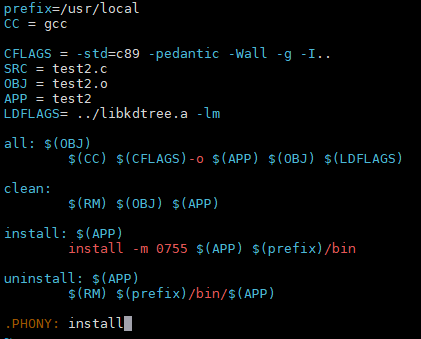
\includegraphics[scale=.72]{imgs/makefile_kdtree.png}
   \caption{Makefile importando librería KD-Tree}
   \label{fig1}
\end{figure}

\subsubsection{Compilación y Prueba del programa}

Se procede a compilar con make y ejecutar el el programa

\begin{lstlisting}[frame=single]
$ make
$ ./test2
\end{lstlisting}

Como se mencionó anteriormente el programa solicita datos al usuario y luego realiza la búsqueda en un árbol kd-tree generado con números al azar. En la siguiente imagen se muestra su ejecución.

\begin{figure}[!h]
   \centering
   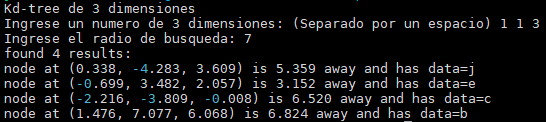
\includegraphics[scale=.72]{imgs/kdtree.png}
   \caption{Ejecución del programa con KD-tree}
   \label{fig2}
\end{figure}
\newpage

\subsection{Compilando el Kernel}

\subsubsection{Descarga y Configuración}

Primero es necesario saber que versión del kernel viene instalada en nuestro sistema, para ello usamos el siguiente comando.

\begin{lstlisting}[frame=single]
$ uname -a
Linux admSist6 4.19.0-10-amd64 #1 SMP Debian 4.19.132-1 (2020-07-24) x86_64 GNU/Linux
\end{lstlisting}

Ahora se procede a descargar la última version estable del kernel

\begin{lstlisting}[frame=single]
$ wget https://cdn.kernel.org/pub/linux/kernel/v5.x/linux-5.8.14.tar.xz
\end{lstlisting}

Se descomprime el paquete

\begin{lstlisting}[frame=single]
$ tar axvf linux-5.8.14.tar.xz
\end{lstlisting}

En caso de haber realizado otra configuración en el actual directorio, es necesario limpiar con los siguientes comandos.

\begin{lstlisting}[frame=single]
$ make distclean
$ make clean
\end{lstlisting}

Luego se debe copiar la configuración con la cuál se configuró el kernel instalado en nuestra máquina.
\begin{lstlisting}[frame=single]
$ cp /boot/config-4.19.0-10-amd64 .config
\end{lstlisting}

Ahora se carga esta configuración anterior para el nuevo kernel
\begin{lstlisting}[frame=single]
$ yes "" | make oldconfig
\end{lstlisting}

En este caso puede arrojar algunos errores de dependencias, en este caso fue necesario instalar flex y bison

\begin{lstlisting}[frame=single]
$ apt install flex
$ apt install bison
\end{lstlisting}

También se puede desplegar un menú en la consola para ver todas las opciones de configuración 
\begin{lstlisting}[frame=single]
$ make menuconfig
\end{lstlisting}

\newpage
\begin{figure}[!h]
   \centering
   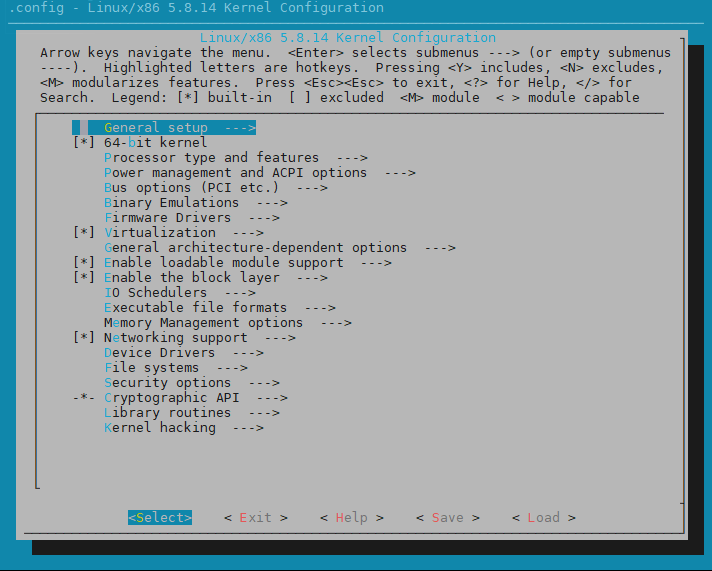
\includegraphics[scale=.39]{imgs/config_kernel2.png}
   \caption{Menú de Configuración del Kernel}
   \label{fig3}
\end{figure}

Se deben seleccionar las opciones dependiendo del cada sistema y los requerimientos. Para este caso se cambio la configuración específica al tipo de CPU y se desactivó drivers de audio que no serán utilizados.

\begin{figure}[!h]
   \centering
   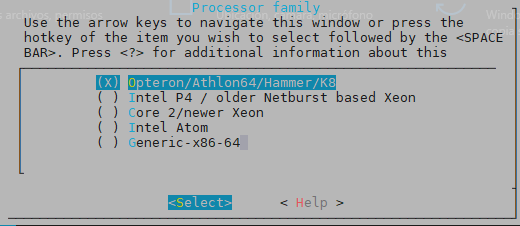
\includegraphics[scale=.40]{imgs/conf_kernel3.png}
   \caption{Configuración de la familia del CPU}
   \label{fig4}
\end{figure}

Una vez configurado se guarda todo y si vemos el contenido del archivo .config se encuentran todos los parámetros de configuración para instalar el nuevo kernel.

\begin{figure}[!h]
   \centering
   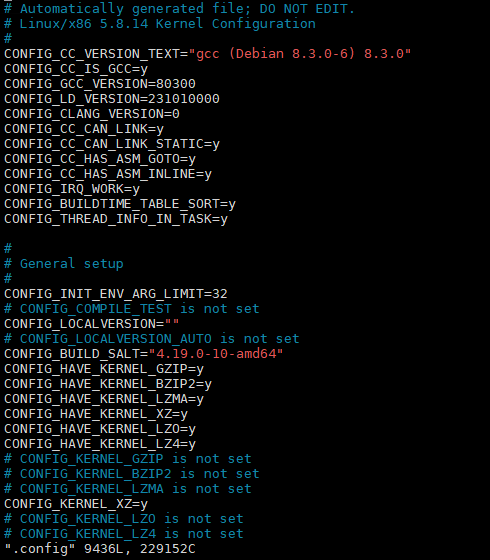
\includegraphics[scale=.39]{imgs/conf_kernel.png}
   \caption{Archivo de Configuración del Kernel}
   \label{fig5}
\end{figure}

Dentro de este archivo es importante modificar la línea que hacer referencia al certificado del kernel anterior.
\begin{lstlisting}[frame=single]
$ nano .config
CONFIG_SYSTEM_TRUSTED_KEYS=""
\end{lstlisting}

Además se puede deshabilitar la línea que crea una imagen dbg con la información del debug del kernel, esto permite que la imagen sea mucho más pequeña y así no quedarse sin espacio durante la compilación.


\begin{lstlisting}[frame=single]
$ nano .config
CONFIG_DEBUG_INFO=n
\end{lstlisting}

\subsubsection{Screen y Compilación}
Ahora quedaría compilar el kernel, para lo cual se hizó una prueba en dos máquinas , una alojada en un servidor remoto y otra localmente. 

\begin{itemize}
\item La máquina remota cuenta con 2 CPUs con 2 hilos de AMD a 2.7 GHz y 2 GB RAM 
\item La máquina local cuenta con 8 CPUs  con 16 hilos de Intel a 5.0 GHz y 16 GB RAM
\end{itemize}

Para la máquina remota se configuró el uso de screen que es un software de terminales virtuales que permiten dejar el proceso de compilación corriendo sin necesidad de estar conectado todo el tiempo al servidor remoto.

Instalación de screen
\begin{lstlisting}[frame=single]
$ apt install screen
\end{lstlisting}

Se crea una terminal en screen con nombre
\begin{lstlisting}[frame=single]
$ screen -S kernel
\end{lstlisting}

Esto nos deja lista la terminal para lanzar un proceso de larga duración en nuestro servidor remoto. Para salir se esta terminal se debe apretar CTR + A + D. Para volver a la terminal creada se pueden listar las terminales de screen creadas
\begin{lstlisting}[frame=single]
$ screen -ls
There is a screen on:
        30906.kernel    (10/10/2020 07:47:05 PM)        (Detached)
1 Socket in /run/screen/S-root.
\end{lstlisting}

Con esto podemos volver a conectarnos a esa terminal
\begin{lstlisting}[frame=single]
$ screen -r 30906.kernel
\end{lstlisting}

Finalmente dejamos corriendo la compilación del kernel
 
\begin{lstlisting}[frame=single]
$ make -j2 deb-pkg
\end{lstlisting}


Para la máquina local se usó 
\begin{lstlisting}[frame=single]
$ make -j16 deb-pkg
\end{lstlisting}

Los tiempos de ejecución en la máquina remota fueron los siguientes
\begin{lstlisting}[frame=single]
real    96m49.182s
user    168m48.511s
sys     20m3.484s
\end{lstlisting}

Mientras que en la máquina local
\begin{lstlisting}[frame=single]
real    11m7.837s
user    129m13.261s
sys     16m43.976s
\end{lstlisting}

\subsubsection{Instalación de la imagen}

Una vez terminado el proceso de compilación solo quedaría instalar la imagen .deb generada
\begin{lstlisting}[frame=single]
$ cd ..
$ dpkg -i dpkg -i linux-image-5.8.14_5.8.14-1_amd64.deb
\end{lstlisting}

Terminada la instalación se reinicia la máquina para que arranque con el nuevo kernel. 
\begin{lstlisting}[frame=single]
$ shutdown -r now
\end{lstlisting}
Si la máquina vuelve arrancar se puede verificar el kernel instalado
\begin{lstlisting}[frame=single]
$ uname -a
Linux admSist6 5.8.14 #1 SMP Sun Oct 11 04:00:29 -03 2020 x86_64 GNU/Linux
\end{lstlisting}
\newpage
\section{Acceso Remoto}
\subsection{Telnet}

Primero es necesario la instalación de telnet
\begin{lstlisting}[frame=single]
$ sudo apt install telnetd
\end{lstlisting}

Una vez instalado se debe correr el servicio para poder utilizarlo
\begin{lstlisting}[frame=single]
$ sudo systemctl start inetd
\end{lstlisting}

Antes de establecer una conexión a otra máquina de forma remota, es necesario crear un nuevo usuario y asignándole un directorio y una contraseña.

Para crear un usuario y asignarle un directorio en /home usamos el siguiente comando.

\begin{lstlisting}[frame=single]
$ sudo useradd -m -s /bin/bash nirojas
\end{lstlisting}

Luego para asignarle una contraseña 

\begin{lstlisting}[frame=single]
$ sudo passwd nirojas
New password:
Retype new password:
passwd: password updated successfully
\end{lstlisting}

Ahora ya podremos conectarnos mediante telnet
\begin{lstlisting}[frame=single]
$ telnet 10.1.1.33 -l nirojas
Trying 10.1.1.33...
Connected to 10.1.1.33.
Escape character is '^]'.
Password:
\end{lstlisting}

\subsection{SSH}

SSH es un protocolo que permite al igual que telnet permite la conexión remota a otra máquina, la diferencia es que SSH utiliza un canal seguro, usando un sistema de cifrado para enviar y recibir la información.\cite{ssh}

\subsubsection{Configuración SSH}

Para conectarse por ssh a un host remoto es necesario especificar el usuario seguido de la dirección ip o hostname de la máquina remota.

\begin{lstlisting}[frame=single]
$ ssh nirojas@bioinfo.utalca.cl
nirojas@bioinfo.utalca.cl's password:
\end{lstlisting}

Para facilitar el ingreso se puede modificar el archivo config ( crear si no existe), para crear un alias a la conexión remota.
\begin{lstlisting}[frame=single]
$ vim .ssh/config

Host bioinfo
user nirojas
hostname bioinfo.utalca.cl
\end{lstlisting}

Además es posible generar una llave encriptada rsa para acceder al host remoto sin indicar la contraseña cada vez que se intente conectar.

Primero se genera una llave rsa que permitirá identificar a nuestro usuario y máquina local.

\begin{lstlisting}[frame=single]
$ ssh-keygen -t rsa
Generating public/private rsa key pair.
Enter file in which to save the key (/home/yanrri/.ssh/id_rsa): 
Enter passphrase (empty for no passphrase): 
Enter same passphrase again: 
Your identification has been saved in /home/yanrri/.ssh/id_rsa.
Your public key has been saved in /home/yanrri/.ssh/id_rsa.pub.
The key fingerprint is:
SHA256:OUkuYjpu7B/wQDdGJoWH84L0P+oBUfTHCprmp6UMTlQ yanrri@CEBOYAN
The key's randomart image is:
+---[RSA 2048]----+
|  o*+            |
| .=+o .          |
|.ooE+. o.        |
|..*+o.oo o       |
| *o.+.. S        |
|+ .* + . .       |
|.+o++ .          |
|=.Bo..           |
| B+o.            |
+----[SHA256]-----+
\end{lstlisting}
  
Luego es necesario crear el directiorio .ssh/ en el host remoto en caso de que no haya sido creado con anterioridad.

\begin{lstlisting}[frame=single]
$ ssh bioinfo mkdir -p .ssh
\end{lstlisting}


Finalemnte se copia la llave generada anteriormente en el archivo que almacena las claves autorizadas para realizar conexión sin password. 
\begin{lstlisting}[frame=single]
$ cat cat ~/.ssh/id_rsa.pub | ssh bioinfo 'cat >> .ssh/authorized_keys'
\end{lstlisting}

\subsubsection{Conexión por túnel}

En algunos casos para conectarse a un equipo, se requiere un host remoto intermedio que haga un túnel al host remoto final.

El host intermedio se puede agregar a la configuración ssh quedando como la siguiente imagen. 

\begin{figure}[!h]
   \centering
   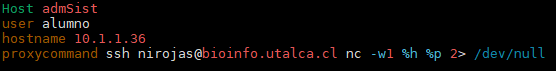
\includegraphics[scale=.82]{imgs/proxy_config.PNG}
   \caption{Archivo config de ssh para establecer conexión remota mediante un túnel}
   \label{fig6}
\end{figure}

La imagen muestra en 'proxycommnad' el host que actua como túnel para establecer la conexión con el host remoto final. En este caso se usa el servidor bioinfo.utalca.cl para poder conectarse a la máquina con dirección IP 10.1.1.36 con el usuario alumno.

Finalmente si se desea conectar a través de un túnel sin indicar contraseña por cada conexión, es necesario copiar la clave rsa tanto en el host intermedio como el host final.

\subsubsection{ SSHFS: Montar archivos remotos}

Otro aspecto interesante de las conexiones remotas es la posibilidad de acceder a los archivos de un host remoto directamente desde nuestra máquina local, para ello existen varias opciones una de ellas es usar el protocolo seguro de SSH con el software SSHFS que permite montar un directorio remoto como se muestra en el siguiente comando.

\begin{lstlisting}[frame=single]
sshfs alumno@10.1.1.36:RemoteFolder/ ~/Documents/ -o ssh_command='ssh -J nirojas@bioinfo.utalca.cl'
\end{lstlisting}

En este caso se agregó la opción \emph{ssh\_command} para lograr la conexión mediante un túnel.

\section{Transferencia de Datos}

\subsection{TFTP}

Corresponde a un protocolo de transferencia de archivos más sencillo y rápido que el clásico FTP ya que realiza un menor número de validaciones y no cuenta con un sistema de cifrado o autenticado. Trabaja sobre el puerto 69 en UDP.\cite{tftp}

Primero será necesario instalar un software que trabaje con este protocolo por el lado del servidor, en este caso se escogió \emph{tftpd-hpa}

\begin{lstlisting}[frame=single]
$ sudo apt install tftpd-hpa
\end{lstlisting}

Una vez instalado se ejecuta el servicio.
\begin{lstlisting}[frame=single]
$ sudo systemctl start tftpd-hpa
\end{lstlisting}

Para comprobar el puerto en el que se esta ejecutando se puede ejecutar el comando netstat

\begin{figure}[!h]
   \centering
   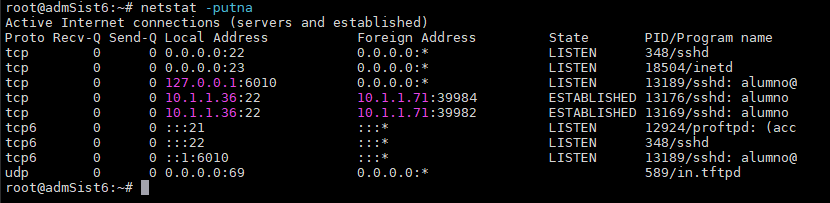
\includegraphics[scale=.69]{imgs/netstat1.png}
   \caption{Puertos de red TCP/UDP en uso}
   \label{fig7}
\end{figure}
Se puede ver que en la última línea el programa tftpd esta usando el puerto UDP 69

Una vez arriba el servidor es necesario instalar un software por el lado del cliente para subir o bajar archivos del servidor. En este caso se instalará  \emph{tftp} .

\begin{lstlisting}[frame=single]
$ sudo apt install tftp
\end{lstlisting}

Para conectarnos al servidor simplemente se debe indicar la dirección IP del servidor tftp
\begin{lstlisting}[frame=single]
$ tftp 10.1.1.35
tftp>
\end{lstlisting}

Se abre una consola en donde se puede digitar el símbolo ? para ver los comandos disponibles.
\begin{lstlisting}[frame=single]
tftp>?
Commands may be abbreviated.  Commands are:

connect         connect to remote tftp
mode            set file transfer mode
put             send file
get             receive file
quit            exit tftp
verbose         toggle verbose mode
trace           toggle packet tracing
status          show current status
binary          set mode to octet
ascii           set mode to netascii
rexmt           set per-packet retransmission timeout
timeout         set total retransmission timeout
?               print help information

\end{lstlisting}
Para enviar un archivo al servidor
\begin{lstlisting}[frame=single]
tftp> put top_secret.txt
Received 15 bytes in 0.0 seconds
tftp>
\end{lstlisting}

Para obtener un archivo que se encuentre en el servidor
\begin{lstlisting}[frame=single]
tftp> get top_secret.txt
Received 15 bytes in 0.0 seconds
tftp>
\end{lstlisting}

\subsection{FTP}

Es el protocolo estándar para la transferencia de archivos. Usa normalmente el puerto 20 y 21 en TCP.

Al igual que con TFTP existen diferentes softwares que implementan este protocolo del lado del servidor y del cliente. Incluso algunas opciones con interfaz gráfica como FileZilla y gFTP. 

En este caso para el servidor se instalará el programa \emph{proftpd}

\begin{lstlisting}[frame=single]
$ sudo apt install proftpd-basic
\end{lstlisting}

Una vez instalado se puede levantar el servicio
\begin{lstlisting}[frame=single]
$ sudo systemd start proftpd.service
\end{lstlisting}

En la Figura \ref{fig7} se puede ver también que el servicio proftpd esta trabajando en el puerto 21 en TCP. 

Con el servidor funcionando podemos instalar el programa \emph{ftp} del lado del cliente.

\begin{lstlisting}[frame=single]
$ sudo apt install ftp
\end{lstlisting}

Para conectarse simplemente se debe indicar la dirección IP del servidor.
\begin{lstlisting}[frame=single]
ftp 10.1.1.35
Connected to 10.1.1.35.
220 ProFTPD Server (Debian) [::1]
Name (10.1.1.35:alumno): nico
331 Password required for alumno
Password:
230 User nico logged in
Remote system type is UNIX.
Using binary mode to transfer files.
ftp>
\end{lstlisting}

En este caso pide una autenticación a través de un usuario y contraseña. Se puede configurar el servidor para permitir conexiones anónimas. Para esto es necesario configurar el archivo de configuración ubicado en \emph{/etc/proftpd/proftpd.conf}

\begin{figure}[!h]
   \centering
   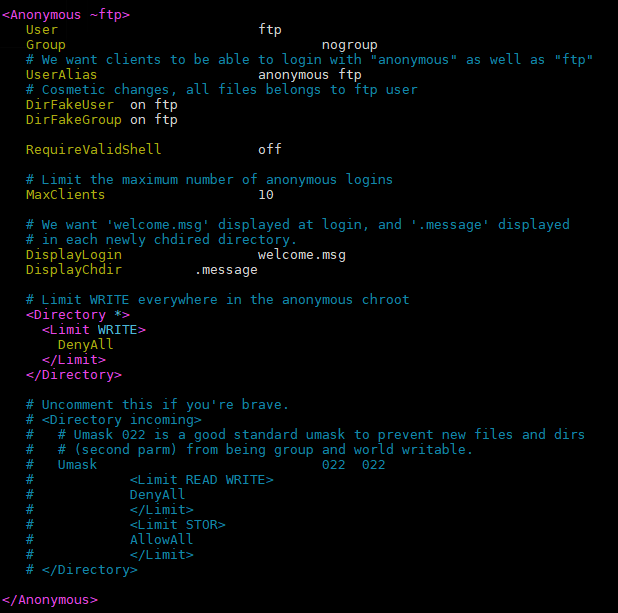
\includegraphics[scale=.39]{imgs/ftp_conf.PNG}
   \caption{Configuración de proftpd para usuarios anónimos}
   \label{fig8}
\end{figure}
Estas líneas estarán comentadas por defecto en el archivo de configuración, al modificar esto será necesario reiniciar el servicio para aplicar los cambios.

\begin{lstlisting}[frame=single]
$ sudo systemctl restart proftpd.service
\end{lstlisting}

Al conectarse simplemente debe especificarse el usuario ftp y omitir la contraseña.
\begin{lstlisting}[frame=single]
$ ftp 10.1.1.35
Connected to 10.1.1.35.
220 ProFTPD Server (Debian) [::ffff:10.1.1.36]
Name (10.1.1.36:alumno): ftp
331 Anonymous login ok, send your complete email address as your password
Password:
230-Welcome, archive user ftp@stgo-10.1.1.35.in.utalca.cl !
230-
230-The local time is: Mon Nov 16 00:22:33 2020
230-
230-This is an experimental FTP server.  If you have any unusual problems,
230-please report them via e-mail to <root@admSist6>.
230-
230 Anonymous access granted, restrictions apply
Remote system type is UNIX.
Using binary mode to transfer files.
ftp> 
\end{lstlisting}

En este caso ftp tiene más opciones que tftp como por ejemplo navegar entre directorios o listar los archivos. Para ver todos los comandos disponibles se puede ver de la misma forma que tftp.

\begin{lstlisting}[frame=single]
>ftp ?
Commands may be abbreviated.  Commands are:

!               dir             mdelete         qc              site
$               disconnect      mdir            sendport        size
account         exit            mget            put             status
append          form            mkdir           pwd             struct
ascii           get             mls             quit            system
bell            glob            mode            quote           sunique
binary          hash            modtime         recv            tenex
bye             help            mput            reget           tick
case            idle            newer           rstatus         trace
cd              image           nmap            rhelp           type
cdup            ipany           nlist           rename          user
chmod           ipv4            ntrans          reset           umask
close           ipv6            open            restart         verbose
cr              lcd             prompt          rmdir           ?
delete          ls              passive         runique
debug           macdef          proxy           send
\end{lstlisting}
\break
Ejemplo para descargar un archivo del servidor
\begin{lstlisting}[frame=single]
>ftp get welcome.msg
local: welcome.msg remote: welcome.msg
200 PORT command successful
150 Opening BINARY mode data connection for welcome.msg (170 bytes)
226 Transfer complete
170 bytes received in 0.00 secs (3.3776 MB/s)
ftp>
\end{lstlisting}


\subsubsection{SSL/TLS: Cifrar el tráfico de FTP}

Otra de las grandes diferencias que tiene FTP con respecto a TFTP es que permite configurar conexiones seguras a través de un certificado  SSL (capa de sockets seguros). Esto permite que la información que se transmite esta cifrada por lo que cualquier persona que intente interceptar el tráfico no podrá acceder ni modificar los archivos. TSL corresponde a una versión actualizada de SSL con mayor seguridad. 

Lo primero es incluir el archivo de configuración para TSL descomentando la siguiente linea.
\begin{lstlisting}[frame=single]
Include /etc/proftpd/tls.conf
\end{lstlisting}

Si es necesario se debe crear el archivo tsl.conf en el directorio \emph{/etc/proftpd/}. Dentro debe estar lo siguiente:
\begin{lstlisting}[frame=single]
# vim tsl.conf
<IfModule mod_tls.c>
     TLSEngine on
     TLSLog /var/log/proftpd/tls.log
     TLSProtocol SSLv23
     TLSRSACertificateFile /etc/ssl/certs/proftpd.crt
     TLSRSACertificateKeyFile /etc/ssl/private/proftpd.key
     TLSRequired on
</IfModule>
\end{lstlisting}
\break
\break
\break
\break
Ahora hace falta generar los certificados público y privado.
\begin{lstlisting}[frame=single]
# proftpd-gencert
Generating a RSA private key
........+++++
.......+++++
writing new private key to '/etc/ssl/private/proftpd.key'
-----
You are about to be asked to enter information that will be incorporated
into your certificate request.
What you are about to enter is what is called a Distinguished Name or a DN.
There are quite a few fields but you can leave some blank
For some fields there will be a default value,
If you enter '.', the field will be left blank.
-----
Country Name (2 letter code) [AU]:CL
State or Province Name (full name) [Some-State]:Maule
Locality Name (eg, city) []:Curico
Organization Name (eg, company) [Internet Widgits Pty Ltd]:Utalca
Organizational Unit Name (eg, section) []:Bioinformatica
Common Name (e.g. server FQDN or YOUR name) []:Nicolas
Email Address []:nicrojas16@alumnos.utalca.cl

Use the following information in your ProFTPD configuration:

TLSRSACertificateFile    /etc/ssl/certs/proftpd.crt
TLSRSACertificateKeyFile /etc/ssl/private/proftpd.key

See /etc/proftpd/tls.conf for suggested TLS related configuration
items and include that file in your /etc/proftpd/proftpd.conf file.
\end{lstlisting}

Por último se reinicia el servicio de proftpd.
\begin{lstlisting}[frame=single]
# systemctl restart proftpd.service
\end{lstlisting}

Para probar la conexión es necesario un cliente con soporte para conexiones seguras como lo es lftp.

Para instalar lftp
\begin{lstlisting}[frame=single]
$ sudo apt install lftp
\end{lstlisting}

Para conectarnos al servidor 
\begin{lstlisting}[frame=single]
$ lftp sftp://alumno@10.1.1.35
Password:
lftp alumno@10.1.1.35:~> get hola.txt
13 bytes transferred
\end{lstlisting}

\section{Resolución de Nombres - DNS}

Con el crecimiento exponencial de las redes en internet han surgido algunos problemas para ubicar y memorizar las direcciones IP de cada uno de los servicios que vistamos en la web. Para ello la solución fue asignar nombres a cada uno de los servicios web para que sea mucho más fácil de recordar y promocionar que una dirección IP, con ello nacen nombres de dominio como google.com, facebook.com, twitter.com, etc. Estos nombres son traducidos a la dirección IP correspondiente mediante un software alojado en un servidor. Por lo tanto cuando nos conectamos a google.com por ejemplo, lo primero que se realiza es mandar la solicitud al servidor DNS para que traduzca este nombre, este nos devuelve la dirección IP del sitio web y a través de esta nos conectamos.  

El software que se utiliza para hacer esta traducción es \emph{bind9}. A continuación se muestra su instalación junto con herramientas para comprobar su funcionamiento.

\begin{lstlisting}[frame=single]
$ sudo apt install bind9 dnsutils dnstracer 
\end{lstlisting}

Una vez instalado se debe configurar y crear los archivos en la carpeta \emph{/etc/bind/} para añadir un nuevo dominio y subdominios.

Para añadir se puede copiar el archivo db.local a otro con el nombre del dominio que vamos a crear por ejemplo db.nicrojas.cl

\begin{lstlisting}[frame=single]
# cd /etc/bind/ 
# cp db.local db.nicrojas.cl
# vim db.nicrojas.cl
\end{lstlisting}

Ahora se debe editar el archivo y se debe cambiar el nombre localhost por el nombre de dominio y subdominio a crear. En la parte final del archivo se debe especificar la IP a la que hace referencia estos nombres, primero el dominio y luego los subdominios como se muestra en la Figura \ref{fig9}.

\begin{figure}[!h]
   \centering
   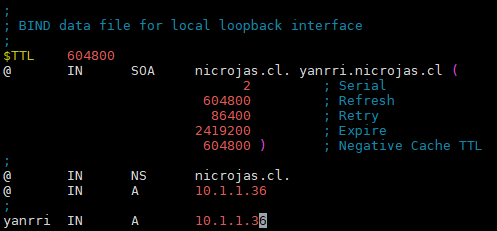
\includegraphics[scale=.65]{imgs/dns_1.PNG}
   \caption{Configuración de archivo db.nicrojas.cl}
   \label{fig9}
\end{figure}

En este caso se configuró que el subdominio este alojado a la misma máquina que el dominio principal pero eventualmente podríamos tener cada subdominio en alguna máquina dedicada para este.

El siguiente archivo a crear es el de named.conf.nicrojas.cl el cual indica la zona con nuestro nombre de dominio e icluye la ruta del archivo db.nicrojas.cl

La estructura de este nuevo archivo es de la siguiente forma:
\begin{lstlisting}[frame=single]
# vim named.conf.nicrojas.cl
zone "nicrojas.cl" {
        type master;
        file "/etc/bind/db.nicrojas.cl";
};
\end{lstlisting}

Por último en el archivo named.conf se encuentran todas las zonas de nuestro servidor DNS, por lo que hay agregar la siguiente línea para agregar el dominio creado.

\begin{lstlisting}[frame=single]
# echo "include \"/etc/bind/named.conf.nicrojas.cl\";" >> /etc/bind/named.conf
\end{lstlisting}

Una vez realizado esto se debe reiniciar el servicio para actualizar las configuraciones.
\begin{lstlisting}[frame=single]
# systemctl restart bind9
\end{lstlisting}

Para comprobar el funcionamiento del dominio podemos conectarnos a la máquina de Jessica(10.1.1.35) y probar el nombre de dominio y subdominio creado.

\begin{lstlisting}[frame=single]
$ ssh nico@10.1.1.35
\end{lstlisting}

Dentro de esta máquina debemos indicar la dirección IP del servidor DNS a utilizar, para ello se debe modificar el archivo \emph{/etc/resolv.conf} y agregar la siguiente línea.

\begin{lstlisting}[frame=single]
# vim /etc/resolv.conf
nameserver 10.1.1.36 
\end{lstlisting}

La línea debe agregarse arriba del resto de nameserver, para que funcione correctamente.

Por último probamos su funcionamiento con la funcionalidad nslookup obteniendo lo siguiente.
\begin{lstlisting}[frame=single]
$ nslookup nicrojas.cl
Server:         10.1.1.36
Address:        10.1.1.36#53

Name:   nicrojas.cl
Address: 10.1.1.36
\end{lstlisting}

Se prueba también el subdominio.
 \begin{lstlisting}[frame=single]
$ nslookup yanrri.nicrojas.cl
Server:         10.1.1.36
Address:        10.1.1.36#53

Name:   yanrri.nicrojas.cl
Address: 10.1.1.36
\end{lstlisting}

Como se puede observar la consulta de nombre la hace al servidor DNS alojado en nuestra máquina remota (10.1.1.36), usando el puerto 53 que es el predeterminado para este servicio. Por último entrega la dirección a la que hace referencia el dominio/subdominio que en este caso corresponde a la misma del servidor DNS.

Otra prueba interesante es poder hacer ping usando el nombre de dominio/subdominio.
 \begin{lstlisting}[frame=single]
$ ping yanrri.nicrojas.cl -c 4
PING yanrri.nicrojas.cl (10.1.1.36) 56(84) bytes of data.
64 bytes from 10.1.1.36 (10.1.1.36): icmp_seq=1 ttl=64 time=0.106 ms
64 bytes from 10.1.1.36 (10.1.1.36): icmp_seq=2 ttl=64 time=0.193 ms
64 bytes from 10.1.1.36 (10.1.1.36): icmp_seq=3 ttl=64 time=0.192 ms
64 bytes from 10.1.1.36 (10.1.1.36): icmp_seq=4 ttl=64 time=0.195 ms

--- yanrri.nicrojas.cl ping statistics ---
4 packets transmitted, 4 received, 0% packet loss, time 54ms
rtt min/avg/max/mdev = 0.106/0.171/0.195/0.040 ms
\end{lstlisting}

\section{Sistema de Archivos por Red: NFS}

NFS es otro protocolo, mediante el cual se pueden compartir archivos de forma distribuida, rápida y sencilla mediante el uso de la red. Sin embargo, no es un protocolo con cifrado ya que busca la mayor rapidez posible en el acceso a los archivos. Debido a esto suele implementarse en entornos de red privados para evitar problemas de seguridad. \cite{nfs}


Primero se debe configurar el servidor principal que alojará la carpeta compartida en la red. Para ello es necesario instalar \emph{nfs-kernel-server}

\begin{lstlisting}[frame=single]
$ sudo apt install nfs-kernel-server
\end{lstlisting}

Luego como root se puede crear una carpeta la que será configurada para ser compartida en la red.
\begin{lstlisting}[frame=single]
# mkdir /NFS_Folder
\end{lstlisting}

Luego en el archivo \emph{/etc/exports} se debe agregar la carpeta creada junto con las dirección IP que tendrá acceso a esta con los permisos. 
\begin{lstlisting}[frame=single]
# vim /etc/exports
/NFS_Folder		10.1.1.0/24(rw,sync,no_subtree_check)
\end{lstlisting}
En este caso se ha configurado para que se pueda compartir con toda la red privada especificando una máscara de subred de /24 bits.

Solo queda reiniciar el servicio para guardar las configuraciones.
\begin{lstlisting}[frame=single]
# systemctl restart nfs-kernel-server.service
\end{lstlisting}

Ahora por parte del cliente es necesario instalar \emph{nfs-common} para montar la carpeta compartida en red.
\begin{lstlisting}[frame=single]
$ sudo apt install nfs-common
\end{lstlisting}

Se crea una carpeta en donde se montará la carpeta compartida
\begin{lstlisting}[frame=single]
$ mkdir shared/
\end{lstlisting}

Como root se monta la carpeta compartida creada en el servidor, sobre la carpeta creada en el cliente. 
\begin{lstlisting}[frame=single]
# mount -t nfs4 10.1.1.35:/shared_Nico /home/alumno/shared/
\end{lstlisting}

Para esto se usó como servidor la máquina de Jessica(10.1.1.35) en dónde se creo la carpeta compartida \emph{shared\_Nico} la cual contiene un archivo para probar su funcionamiento. Una vez montado en el cliente(10.1.1.36) se ven los archivos en ambos lados.
\bigskip
\begin{lstlisting}[frame=single]
root@admSist5:/shared_Nico# ls
soy_un_archivo.txt
\end{lstlisting}

\begin{lstlisting}[frame=single]
alumno@admSist6:~/shared$ ls
soy_un_archivo.txt
\end{lstlisting}

\subsection{Cambiar permisos de la carpeta compartida}

Con las configuraciones anterior solamente el servidor podrá editar/modificar los archivos, mientras que el cliente solo tendrá acceso de lectura, esto pese a que en la configuración de \emph{/etc/exports} tenga permisos para escribir también. Para revertir esto será necesario cambiar permisos también a la carpeta creada en el servidor y también se puede agregar a la configuración que los archivos queden con propietario de un usuario.

Para asignar los permisos a la carpeta compartida
\begin{lstlisting}[frame=single]
# chmod 777 /shared_Nico/
# chmod u+rwx /shared_Nico/
\end{lstlisting}

Cambiar propietario a la carpeta compartida y sus archivos 
\begin{lstlisting}[frame=single]
# chown alumno:alumno -R shared_Nico/
\end{lstlisting}

Asignar el propietario desde configuración NFS.
\begin{lstlisting}[frame=single]
# vim /etc/exports
/home/alumno/shared_Nico 10.1.1.36(rw,sync,no_subtree_check,anonuid=1000,anongid=1000)
\end{lstlisting}
En este caso se agrega el uid del usuario que quedará como propietario de los archivos que se agreguen a la carpeta compartida.

Para ver la información e id de los usuarios de la máquina.
\begin{lstlisting}[frame=single]
$ cat /etc/passwd
\end{lstlisting}
\subsection{Montar automáticamente}

Una vez todo configurado pareciera estar listo una vez que se realiza el montaje, sin embargo al apagar o reiniciar la máquina es necesario volver a montar la carpeta compartida en la red. Esto se puede cambiar configurando el automontaje.


Por ejemplo al reiniciar y luego listar los archivos de la carpeta en dónde se había realizado anteriormente el montaje, se puede ver que esta se encuentra vacía.
\begin{lstlisting}[frame=single]
# shutdown -r now
$ cd ~/shared
$ ls -ll
total 0
\end{lstlisting}
\newpage
Para montar de forma automática es necesario editar como root el archivo \emph{/etc/fstab} .
\begin{lstlisting}[frame=single]
# vim /etc/fstab
\end{lstlisting}

Dentro del archivo se agrega la información del montaje primero la IP del servidor con la ruta de la carpeta y luego la carpeta local en dónde se hará el montaje. Luego una serie de parámetros como se ve en la siguiente figura. 

\begin{figure}[!h]
   \centering
   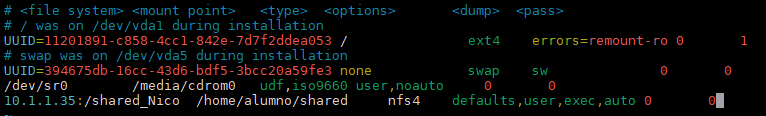
\includegraphics[scale=.85]{imgs/nfs_auto.PNG}
   \caption{Configuración de archivo /etc/fstab}
   \label{fig10}
\end{figure}

El parámetro que permite el montaje automático es el de \emph{auto}. Con esto guardamos el contenido del archivo y podemos comprobar reiniciando nuevamente y debería estar montado con los archivos compartidos en red.

\begin{lstlisting}[frame=single]
# shutdown -r now
$ cd ~/shared
$ ls -ll
total 4
-rw-r--r-- 1 root root 49 Nov 22 05:14 soy_un_archivo.txt
\end{lstlisting}

Para desmontar la unidad simplemente con el comando \emph{umount}.

\begin{lstlisting}[frame=single]
# umount /home/alumno/shared
\end{lstlisting}

 Sin embargo para que no se vuelva a montar cuando se reinicie la máquina será necesario modificar el archivo \emph{/etc/fstab} en el parámetro \emph{auto} por \emph{noauto}.
%--------------%
\newpage
\begin{thebibliography}{99}
\bibitem{mlinux} Manual Linux \url{https://manualinux.eu/gcc.html}
\bibitem{ssh} SSH \url{https://es.wikipedia.org/wiki/Secure_Shell}
\bibitem{tftp} TFTP \url{https://es.wikipedia.org/wiki/TFTP}
\bibitem{nfs} NFS \url{https://www.extrahop.com/resources/protocols/nfs/}
\end{thebibliography}
\end{document}
